\documentclass[template.tex]{subfiles}
\begin{document}

\xchapter{Fundamentação Teórica e revisão da literatura}{}

%\begin{itemize}
%\item A área de mineração de opiniões é recente (Pang and Lee, 2008);
%\item Tão recente que ainda existem problemas de terminologias (mineração de opinião, análise de sentimentos, mineração de sentimentos, análise afetiva, dentre outros);
%\item Definição de opinion mining (usar um cara forte para isso, como Lib Bing, Po Pang, Turney, etc.)
%
%\item Definição formal de opinião 'O':
%\begin{itemize}
%\item O = (g, s), onde \emph{g} é o alvo e \emph{s} é o sentimento associados a opinião
%\end{itemize}
%
%\item Níveis de mineração de opinião (cita e depois explica cada um deles e diz qual foi usado e por que. Além de, claro, falar de trabalhos que se encaixam em cada nível)
%\begin{itemize}
%\item Nível de documento;
%\item Nível de sentença;
%\item Nível de entidades e seus aspectos
%\end{itemize}
%
%\item angelo: apresente uma visão dos problemas de pesquisa da área (classificação de polaridade, subjetividade, etc), por ser por exemplificação se não tiver uma referência que faça um review sobre isso
%
%\item angelo: precisa falar sobre a etapa de pré-processamento e transformação, e daí comenter sobre as abordagens baseada em bag-of-words e baseada em features 
%
%\item angelo: comente em algum lugar sobre as abordagens baseada em bag-of-words e baseada em features 
%
%\item Lógica Fuzzy
%\begin{itemize}
%\item Muitas das informações que lidamos são imprecisas e vagas;
%\item A lógica clássica não consegue lidar com esse tipo de informação;
%\item Para isso,Zadeh (1965) propôs a Lógica Nebulosa para lidar com informações vagas e imprecisas
%
%\item Conjuntos Fuzzy
%\begin{itemize}
%\item A lógica nebulosa diz que um elemento pode fazer parte de mais de um conjunto com graus de pertinência para cada um deles (Uma opinião pode ser positiva e negativa ao mesmo tempo, mas com graus de pertinência para cada conjunto fuzzy)
%\item A lógica clássica, por outro lado, determina que um objeto pertençe ou não a um conjunto (Ou uma opinião é positiva ou negativa);
%\end{itemize}
%
%\item Wang-Mendel
%\begin{itemize}
%\item O que é?
%\item Explicar o método
%\end{itemize}
%
%\item Fala de outros algoritmos de classificação e agrupamento? Tem isso na qualificação, mas não sei se é mais pertinente (??????)
%
%\item Métodos de classificação com uso de regras
%\begin{itemize}
%\item CFRM
%\item GFRM
%\end{itemize}
%\end{itemize}
%\item Trabalhos relacionados
%\begin{itemize}
%\item Papers with opinion mining? (Angelo: Acho que alguns principais, mais para contextualizar as abordagens, independente e dependente de domínio, classificação com palavras e com features)
%\item Papers with both? (angelo: Sim, descrever rapidamente os encontrados e fazer contraste com a nossa proposta)
%\end{itemize}
%
%\end{itemize}

\section{Mineração de Opinão}

Mineração de opinião é o campo de estudo que analisa as opiniões, sentimentos, avaliações, atitudes e emoções de pessoas direcionadas a entidades ou alvos, como produtos, serviços, organizações, indivíduos, problemas, eventos, tópicos e seus atributos \cite{bing:2012}. A pesquisa em mineração de opinião começou com detecção de subjetividade, com os trabalhos de \citeonline{carbonell1979subjective}, \citeonline{wilks1983beliefs} e \citeonline{wilson2004just}. Essa tarefa envolvia a detecção e separação das sentenças objetivas das subjetivas, que carregam as opiniões e sentimentos atrelados. Com o passar dos anos, começando nos anos 2000, foi que a linha de pesquisa de mineração de opinião alavancou, focando em classificar as opiniões em três categorias: negativo, positivo e neutro. A partir daí muitos trabalhos foram publicados nessa área, mas com diferentes denominações, como análise de sentimentos, mineração de sentimentos, classificação de opiniões, dentre outros. 

Somente em 2003, no trabalho de \citeonline{dave2003mining}, é que o termo mineração de opinião foi usado e, juntamente com análise de sentimento, cunhado por \citeonline{nasukawa2003sentiment}, é que o termo passou a ser largamente adotado. No entanto, atualmente, ambos os termos denotam o mesmo campo de pesquisa \cite{bing:2012, pang:2008}. Sendo assim, neste trabalho, ambos os termos serão utilizados alternadamente, mas, com o objetivo de simplificar a leitura e compreensão deste texto, o termo de mineração de opinião será majoritariamente utilizado.

\section{Níveis de mineração de opinião}

%\todo[inline]{coloca exemplos aqui, pode obter documentos, comentários e sentenças de sites se achar melhor, há somente um exemplo aqui}
%\todo[inline]{matheus: nao entendi direito, mas eu adicionei exemplos em cada paragrafo. Veja se foi isso que quis dizer.}

Mineração de opiniões é uma área de pesquisa que vem sendo investigada em três principais níveis de análise: i) nível de análise de documento, ii) sentenças e iii) entidades e seus aspectos. O primeiro nível foca em classificar uma opinião de um documento expressando-a como positiva ou negativa. O segundo nível, o de sentenças, em vez de considerar o sentimento geral de um documento como todo, classifica as opiniões de cada sentença separadamente. E o último nível foca em descobrir todos os alvos existentes em sentenças e documentos e classificar as opiniões direcionadas a eles \cite{bing:2012}.

O nível de análise de documento é também denominado na literatura como uma tarefa de classificação de sentimentos em nível documento, pois considera todo o documento como uma unidade de informação \cite{bing:2012, pang:2008}. É importante salientar que, nesse nível de detalhamento, é assumido que o documento expressa opiniões direcionadas para somente um único assunto e somente possui um único autor das opiniões. Essa análise é feita normalmente sobre opiniões sobre produtos e serviços, pois cada avaliação, normalmente, foca somente em um único produto ou serviço e é escrito por somente uma pessoa \cite{bing:2012}. Por exemplo, opiniões sobre filmes retiradas do IMDB ou Rotten Tomatoes \footnote{\url{www.rottentomatoes.com/}} ou de produtos da Amazon, são utilizadas nesse nível, pois as opiniões são normalmente direcionadas a somente ao filme ou produto em questão. 

%Um grande número de trabalhos foram publicados na literatura sobre mineração de opiniões em nível de documento. \citeonline{gamon2004sentiment} utilizou opiniões de clientes registradas em pesquisas de opinião como conjunto de dados para mineração de opiniões. Neste trabalho foi utilizado o algoritmo de classificação SVM (\textit{Support Vector Machine}), que produz bons resultados em classificação textual \cite{joachims1998text}. Foram realizados também estudos para identificar quais características textuais eram mais relevantes para o treinamento do SVM e, por conseguinte, para minerar opiniões. \cite{mullen2004sentiment} fizeram um trabalho similar ao de \citeonline{gamon2004sentiment}, utilizando o algoritmo SVM e investigando as características textuais mais relevantes para melhorar a mineração e classificação das opiniões. Estes trabalhos utilizaram opiniões de filmes do site Epinions.com \footnote{Disponível em: http://www.epinions.com/} e opiniões de publicações da Pitchfork Media \footnote{Disponível em: http://pitchfork.com/}.

A mineração de opinião em nível de sentenças é uma abordagem que aumenta a granularidade da análise e determina se cada sentença de um ou mais documentos expressam opiniões positivas, negativas ou neutras. As definições do problema e da suposição principal deste nível são definidas a seguir \cite{bing:2012}: dada uma sentença, deve ser ser determinado quando ela expressa uma opinião positiva, negativa, neutra ou nenhuma opinião, considerando que a sentença deve conter somente uma única opinião de um único autor. Esse nível de análise é bastante utilizado como passo intermediário para o terceiro nível, o nível de entidade e aspectos. Analisando cada sentença individualmente é possível identificar as entidades e quais as opiniões estão sendo direcionadas à elas.  Uma aplicação para o nível de sentenças é na extração de opiniões onde o tema é livre e várias opiniões sobre diferentes assuntos emergem, como em fóruns de discussão e redes sociais. 

%O trabalho de \citeonline{Hu:2004} mostra uma sumarização das opiniões de produtos. Nele, sumarizar significa minerar as características dos produtos que possuem opiniões direcionadas a elas e classificar as opiniões como positivas ou negativas. Primeiramente, as sentenças que continham opiniões eram identificadas, utilizando um conjunto de palavras normalmente usado para expressar opiniões. Em seguida, foi definido o sentimento geral (positivo ou negativo) das opiniões, baseando-se no dicionário Wordnet \footnote{Disponível em: http://wordnet.princeton.edu/}. A sentimento geral de cada sentença foi determinado por um algoritmo específico proposto pelo trabalho. Os resultados obtidos foram comparados somente com trabalhos já realizados pelos próprios autores, os quais foram melhorados.Em \citeonline{kim2004determining} foi realizado um trabalho similar ao de \citeonline{Hu:2004}. Contudo, os autores das opiniões eram identificados.  A determinação do sentimento geral das opiniões encontradas nas sentenças foi feita da mesma forma como proposto por \citeonline{Hu:2004}. A diferença está nos algoritmos propostos que definem a orientação final de cada sentença, pois os autores propuseram três algoritmos de classificação e fizeram a análise de desempenho entre eles.

Também denominado nível de entidade e características, o nível de entidade e aspectos é o último nível de análise em mineração de opinião \cite{bing:2012}. Este nível possui duas tarefas principais \cite{bing:2012}: extração dos alvos das opiniões e a classificação das opiniões referentes a esses alvos. A primeira tarefa consiste em extrair os alvos das sentenças. Por exemplo, na sentença "A qualidade de voz desse telefone é muito boa", o alvo é a qualidade da voz e a entidade é o telefone (mais precisamente "este telefone"). A segunda tarefa consiste em classificar - como positivas, negativas ou neutras - as opiniões referentes aos aspectos e das entidades extraídas. No exemplo anterior, a opinião referente ao aspecto "qualidade de voz" da entidade "este telefone" é positiva \cite{bing:2012}.

%Assim como feito em \citeonline{Hu:2004} e \citeonline{kim2004determining}, o trabalho realizado por \citeonline{ding2008holistic} também focou em minerar opiniões de produtos e suas características. Todavia, este trabalho propôs uma nova abordagem para minerar opinião. Em vez de utilizar, por exemplo, as técnicas associadas ao uso do Wordnet, este trabalho focou em tratar problemas de sentimento geral das palavras levando em consideração o contexto (outras sentenças, outros documentos, distância da opinião referente alvos, dentre outros); tratar conflitos entre opiniões numa sentença (e.g. opiniões contrárias); e utilizar padrões lingüísticos (e.g. regras de negação, clausulas \textit{but}) para tratar palavras especiais, frases e construções verbais. O resultado do artigo é um sistema, chamado de \textit{Opinion Observer}, que produz resultados melhores que os trabalhos relacionados na literatura, como em \citeonline{Hu:2004} e  \citeonline{kim2004determining}.

\section{Etapas na mineração de opinião}

%\todo[inline]{faz uma breve introdução nesta seção, dizendo que o processo de mineração de opinião tipicamente envolve diversas etapas que podem envolver  iniciam por pré-processamento dos dados e em alguns trabalhos por extração de características até alcançar a classificação}
%\todo[inline]{matheus: feito}

O processo de mineração de opinião tipicamente envolve algumas etapas, as quais consistem desde a preparação dos dados dos documentos até a classificação destes. É comum encontrar nos trabalhos relacionados as seguintes etapas para minerar e classificar opiniões:  i) definição do domínio, ii) pré-processamento, iii) transformação, iv) seleção de características, v) classificação e vi) análise dos resultados \cite{moraes2012document}. 

A definição do domínio é a fase em que são selecionadas os tipos de dados que serão utilizados para o estudo, como filmes, hotéis, produtos, etc. O pré-processamento é a etapa em que as bases escolhidas são estruturadas para serem utilizadas nas próximas etapas, como a eliminação de termos indesejados, erros de grafia, dentre outros. A transformação é o momento em que os termos estruturados do pré-processamento são transformados em dados numéricos. A extração e seleção de características envolve a obtenção de características descritivas dos documentos a partir dos dados anteriores, assim como, a seleção das características mais relevantes. É importante destacar que a extração de características não é tão comum de ser encontrada. De fato, é típico encontrar trabalhos que não é feita qualquer extração e a seleção é realizada diretamente sobre os dados oriundos do pré-processamento. A etapa de classificação consiste na classificação dos documentos, utilizando as características selecionadas na etapa anterior. E, por fim, na etapa de avaliação é realizada a análise dos resultados obtidos pelo classificador.

As próximas seções detalharão os principais conceitos envolvidos em cada etapa do processo de mineração de opinião.

\subsection{Pré-processamento dos dados}

Em mineração de opinião, a preparação dos dados é essencial. Antes de os dados serem transformados, analisados, selecionados e, então, classificados, eles precisam ser preparados para serem usados corretamente no processo de mineração de opinião. Textos são dados não estruturados e as opiniões se misturam às porções não opinativas do documento. As principais tarefas envolvidas no pré-processamento são: a marcação gramatical das palavras do texto (do inglês, \textit{Part of Speech Tagging}), definição dos n-grams a serem utilizados e a tokenização das palavras. N-gram é uma seqüência de $n$ itens dada uma seqüência de um texto \cite{dave2003mining}. 

A marcação gramatical das palavras do texto é o processo de identificação das classes gramaticais de todos os elementos textuais do documento \cite{brill1995transformation}. Até o presente momento da pesquisa, todos os artigos encontrados executaram essa tarefa, especificando ou não o tipo do marcador gramatical, como pode ser visto em \citeonline{pang2002thumbs, turney2002thumbs, wilson2005recognizing, chaovalit2005movie}. O marcador utilizado nessa pesquisa, devido a ser o mais usado nos trabalhos relacionados, foi o proposto em \citeonline{brill1995transformation}.

Depois do texto identificado e marcado é preciso definir quais n-grams serão selecionados para a próxima etapa. Adjetivos são centrais para identificar subjetividade e, por conseguinte, opiniões em textos. Em \citeonline{hatzivassiloglou2000effects} foi desenvolvido um algoritmo para determinar o sentimento final somente de adjetivos. Neste trabalho foi notado que há relação entre adjetivos e conjunções, como "but", "and", dentre outros. A conjunção "And", por exemplo, mantem a mesma polaridade da opinião expressa pelo adjetivo, enquanto que "but", essa polaridade é invertida, em geral. Utilizando um algoritmo de aprendizado de máquina, esse artigo conseguiu classificar os adjetivos com acurácias entre 78\% e 92\%, dependendo da quantidade de dados de treino disponíveis. Outros trabalhos como os de \citeonline{wiebe2000learning} também utilizaram somente adjetivos como indicadores de subjetividade e presença de opiniões.

\citeonline{turney2002thumbs}, por sua vez, apontou que adjetivos isolados podem indicar opiniões, mas podem não ser suficientes para determinar o sentimento geral de documentos. Ele ainda considera o contexto como fator determinante, exemplificando que "unpredictable" pode ser uma opinião negativa para automóveis, quando associado a "unpredictable steering" ou positivo quando for direcionado a filmes, quando associado a "unpredictable plot". Assim, \citeonline{turney2002thumbs} expande os adjetivos e acrescenta advérbios, verbos e substantivos associados aos adjetivos, extraindo dos textos os chamados bigrams, n-grams compostos por dois elementos textuais. \citeonline{turney2002thumbs} alcançou uma média de acurácia de 74\% entre opiniões sobre automóveis e filmes. 

%\todo[inline]{não fale sobre nossa proposta ou metodologia aqui, fale de forma mais geral, além disso nós usamos o SWN, então não usamos só o texto. Tem váripos }
%\todo[inline]{matheus: removi e fiz um link rapido do paragrafo anterior com o proximo que fala da transformacao.}
%Contudo, nosso trabalho procura classificar o sentimento geral das opiniões dos documentos sem utilizar qualquer outra informação, exceto os próprios textos. Assim, nosso classificador desconhece que o texto de um dado documento se refere a filmes, hotéis ou automóveis. Os trabalhos de \citeonline{wilson2005recognizing}, \citeonline{benamara2007sentiment}, \citeonline{taboada2008extracting} e \citeonline{taboada2011lexicon}, mostraram que o uso de advérbios associados a adjetivos produzem melhores resultados que o uso isolado de adjetivos. Nesses trabalhos, dentre as diferentes nomenclaturas, os advérbios são chamados de modificadores de intensidade dos adjetivos, aumentando a polaridade do adjetivo ou diminuindo. 
%
%Portanto, como nossa proposta não utiliza contexto e adjetivos e advérbios, associados entre si, são reconhecidamente bons elementos para encontrar e mapear conteúdo opinativo, eles foram escolhidos como os n-grams a serem selecionados na etapa de pré-processamento e enviados para a etapa de transformação.

%\subsection{Transformação}

%- Abordagens de aprendizado supervisionado, em geral, não utilizam técnicas de transformação dos n-grams em valores numéricos, pois eles utilizam os proprios n-grams para o processo de seleção de características.
%
%- Abordagens de aprendizado não-supervisionado utilizam dicionários opinativos
%
%- Os dicionários opinativos podem ser construídos manualmente e automaticamente
%
%- pro e contras dos manuais
%
%- pros e contras dos automaticos
%
%- Sentiwordnet, General Inquirer, dentre outros
%
%- O SWN é mais palavras e maior cobertura
%
%- Tecnicas de transformação: posição do n-gram, frequência do n-gram
%
%- Tecnicas de transformação para n-grams de negação: inversão, shift, bias compensation 

Uma vez definidos os n-grams a serem utilizados no processo de mineração de opinião, é na etapa de transformação que uma representação numérica é computada a partir dos n-grams obtidos da etapa de pré-processamento. Diferentes técnicas são utilizadas na literatura para calcular essa representação numérica dos n-grams. \citeonline{turney2002thumbs}, por exemplo, utilizou uma técnica proposta em \citeonline{turney2001mining} chamada PMI-IR, que utiliza \textit{Pointwise Mutual Information} (PMI) e \textit{Information Retrieval} (IR) para medir a similaridade de pares de palavras ou frases. 

%A polaridade de uma ou par de palavras, assim como foi chamada a representação numérica pelo autor, era calculada comparando a similaridade dos pares de palavras com uma palavra de referência positiva  (\textit{excellent}) e com uma palavra de referência negativa (\textit{poor}). A polaridade do n-gram é negativa se o termo por mais similar à referência negativa e positiva se mais similar à referência positiva. \citeonline{wilson2005recognizing} e \citeonline{voll2007not} utilizaram a mesma técnica de \cite{turney2002thumbs}.

%Em \citeonline{tsutsumi2007movie}, a representação numérica dos n-grams é chamado de escore das palavras. Nesse artigo, o escore de uma palavra $w_i$ foi calculada pela fórmula \ref{eq:w_score}.
%
%\begin{equation}
%Score_w(w_i) = \log(\frac{pos(w_i) + 1}{\sum pos} \cdot \frac{\sum neg}{neg(w_i) + 1})
%\label{eq:w_score}
%\end{equation}
%
%onde $pos(w_i)$ e $neg(w_i)$ são a frequencia de uma palavra $w_i$ em opiniões positivas e negativas, respectivamente. $\sum pos$ e $\sum neg$ são o número de palavras em opiniões positivas e negativas, respectivamente. Se $Score_w$ for maior que zero, a polaridade é positiva, senão negativa.

Já \citeonline{taboada2008extracting}, utilizou de dicionários de opinião, que contém os termos e os respectivos graus opinativos. Contudo, esses dicionários foram criados pelos autores do artigo. \citeonline{ohana2009sentiment}, por outro lado, utilizaram um dicionário criado automaticamente, o Sentiwordnet \cite{esuli2006sentiwordnet}. É um dicionário de opiniões criado pela anotação automática dos sentimentos de cada \textit{synset} (conjuntos de sinônimos) do Wordnet, outro dicionário na língua inglesa \cite{fellbaum2005wordnet}. Segundo \citeonline{ohana2009sentiment}, dicionários manuais estão sujeitos ao enviesamento do autor, possuem alto tempo gasto para construí-los e, em geral, tem menor cobertura que dicionários criados automaticamente. \citeonline{ohana2009sentiment} também citou outros dicionários de opiniões criados automaticamente, como \textit{General Inquirer} \cite{stone1966general} \footnote{Disponível em: \url{http://www.wjh.harvard.edu/~inquirer}}, \textit{Subjectivity Clues} \cite{wilson2005recognizing} e \textit{Grefenstette} \cite{grefenstette2004coupling}, mas mostrou que o Sentiwordnet tem cobertura maior frente a estes, com mais de 28000 termos cobertos, contra 4216, 7650 e 2258 dos dicionários citados, respectivamente. Esta pesquisa decidiu pelo uso do Sentiwordnet \cite{esuli2006sentiwordnet}.

Dicionários opinativos, contudo, somente conseguem definir a polaridade de unigrams, ngrams compostos somente por um termo. Para tratar a definição da polaridade de bigrams e trigrams, por exemplo, é preciso analisar a influência entre os termos que compõem o ngram. Se tratando de advérbios e adjetivos, os advérbios são termos que alteram o grau de polaridade de uma adjetivo, seja intensificando (e.g. \textit{very good}) ou amenizando (e.g. \textit{somewhat sleazy}) \cite{quirk1985comprehensive}. Há também inumeras maneiras de tratar a influência entre os termos num bigram, uma delas, e foi a escolhida para essa pesquisa, foi a de \citeonline{taboada2008extracting}. \citeonline{taboada2008extracting} dividiu os advérbios em amplificadores e amenizadores. Os amplificadores aumentam a polaridade do adjetivo e os amenizadores diminuem. De maneira similar ao que fizeram com os dicionários anteriores, os advérbios tiveram associados, manualmente, percentuais de modificação, onde os amplificadores tem percentuais positivos e os amenizadores, negativos. Por exemplo, \textit{sleazy} tem escore ou polaridade -3 e \textit{somewhat}, um amenizador, tem percentual igual a -30\%. O bigram \textit{somewhat sleazy} terá polaridade final de $-3 + (3 \cdot 30\%) = -2$.

Outro fenômeno referente ao relacionamento entre termos num ngram é a negação. A negação ocorre quando n-grams de negação (e.g. advérbios) se associam a um ou mais n-grams, como \textit{nothing special} ou \textit{not very good}. Há, mais uma vez, diferentes maneiras de se tratar uma negação, como a inversão e o deslocamento de polaridade. A inversão inverte o sinal da polaridade do n-gram (e.g. \textit{not sleazy} resultará na polaridade +3). O deslocamento da polaridade desloca o valor da polaridade do n-gram em direção a polaridade oposta por um valor fixo (na implementação desse artigo, foi defino por 4). Assim, por exemplo, em vez de \textit{not sleazy} resultar em +3, a polaridade resultante será de $-3 + 4 = +1$ \cite{taboada2008extracting}.

Há outras abordagens de transformação das polaridades dos termos relativas ao texto, como a freqüência e ao enviesamento das opiniões \cite{taboada2011lexicon}. O tratamento da frequência de termos é a diminuição da polaridade dos termos opinativos pela quantidade de vezes que eles aparecem no texto, resultando numa polaridade $pol = pol \cdot 1/n$. A repetição de termos opinativos sugere que o autor das opiniões carece de comentários adicionais e se utiliza de uma palavra opiniativa genérica. Além disso, existe uma tendencia natural de seres humanos em favor de uma linguagem positiva \cite{boucher1969pollyanna}, resultando conseqüentemente, no enviesamento na classificação de opiniões baseadas em dicionários \cite{kennedy2006sentiment}. Assim, nós aplicamos um aumento de 50\% sobre qualquer n-gram negado que ocorresse nos textos \cite{taboada2011lexicon}.


%No caso de \citeonline{taboada2008extracting} foram utilizados 4 dicionários: adjetivos, verbos, substantivos e advérbios. Os três primeiros foram criados manualmente, e o último criado automaticamente a partir do dicionário de adjetivos, mas todos eles tiveram seus termos associados, manualmente, a um valor dentro de uma escala entre -5 a 5, onde -5 denota extrema negatividade, 0 sem polaridade (ou neutro) e 5, extrema positividade. Esses dicionários foram criados por um dos autores do artigo, aumentados por outro autor e tiveram a consistência checada por mais três pesquisadores. Diferentemente dos trabalhos de \citeonline{turney2002thumbs} e de \citeonline{tsutsumi2007movie}, \citeonline{taboada2008extracting} tratou o relacionamento entre os n-grams utilizados, como a influência de advérbios sobre os adjetivos, e como eles alteram a polaridade final destes. Nesse artigo, essa influência foi chamada de intensificação.

%Seguindo a classificação feita por \citeonline{quirk1985comprehensive}, 

%Além disso, o trabalho de \citeonline{taboada2008extracting} também tratou o fenômeno da negação. A negação ocorre quando n-grams de negação (e.g. advérbios) se associam a um ou mais n-grams, como \textit{nothing special} ou \textit{not very good}. Há diferentes maneiras de se tratar uma negação, como a inversão e o deslocamento de polaridade, proposto nesse mesmo artigo. A inversão inverte o sinal da polaridade do n-gram (e.g. \textit{not sleazy} resultará na polaridade +3). O deslocamento da polaridade 	desloca o valor da polaridade do n-gram em direção a polaridade oposta por um valor fixo (na implementação desse artigo, foi defino por 4). Assim, por exemplo, em vez de \textit{not sleazy} resultar em +3, a polaridade resultante será de $-3 + 4 = +1$.

 
%
%\citeonline{ohana2009sentiment} também trata a negação, usando uma versão do algoritmo \textit{NegEx} \cite{chapman2001evaluation}, embora não trate dos intensificadores e amenizadores. Todavia, \citeonline{ohana2009sentiment} apresenta o conceito de que a polaridade de um termo pode ser maior ou menor a depender de sua posição no texto. A polaridade do termo é alterada conforme mostrado na equação \ref{eq:adj_score}.
%
%\begin{equation}
%Score_{adj} = Score_{adj} \cdot \frac{t_i}{T} \cdot C
%\label{eq:adj_score}
%\end{equation}
%
%Onde $C$ é uma constante, $t_i$ a posição do termo $t$ relativa ao total de termos $T$ no documento.

\subsection{Extração e seleção de características}

%- Poucos trabalhos foram encontrados que extraem características
%
%- Que trabalhos foram esses, quais tipos de caracteristicas eles extrairam, como fizeram e o que fizeram com elas?
%
%- Selecao de caracteristicas é a etapa de selectionar melhores caracteristicas e diminuir a dimensionalidade dos vetores para melhorar a performance da classificacao
%
%- Não ha metodo de selecao de caracteristica que tenha se mostrado predominante na linha de pesquisa. Information Gain parece ser promissor. (Rodrigo Morais)
%
%- Cita trabalhos que fizeram seleção, qual tecnica usaram, como fizeram e como utilizaram
%
%- Cita tambem o trabalho que usou o CFS e o C45

%\subsection{Extração de características}

%\todo[inline]{precisa criar coesão com mineração de opinião, começa (ficou truncado) }
%\todo[inline]{matheus: voce alterou aqui? pq senao, eu n entendi onde não tem a coesão}

Usualmente, os dados da etapa de transformação já são considerados as características e são utilizados diretamente na seleção. Porém, uma etapa adicional poderia ser a extração de características dos documentos, que consiste em obter as características que caracterizam os documentos, independentemente do conteúdo específico destes. Essa é uma etapa encontrada em poucos trabalhos relacionados nessa linha de pesquisa. Os trabalhos de \citeonline{wilson2005recognizing} e de \citeonline{ohana2009sentiment} foram um dos poucos encontrados na literatura que definiram e extraíram as características dos documentos, e posteriormente, as utilizaram para a classificação dos mesmos.
%\todo[inline]{esse comentário sobre 'nossa pesquisa', deve ficar na metodologia}
%\todo[inline]{matheus: comentario jaz}
%Nossa pesquisa utilizou grande parte das categorias de características de \citeonline{ohana2009sentiment} para definir e extrair as nossas próprias.

%Em \citeonline{wilson2005recognizing}, que foca em classificar o sentimento geral das opiniões em nível de sentenças, definiu 5 categorias de características: palavras, modificação, estrutura, sentença e documento. As características de palavras e de modificação são os próprios n-grams, nesse caso, trigrams, uma sequência de três palavras num outra sequencia textual. \citeonline{wilson2005recognizing} estrutura os documentos numa árvore de dependencia entre os elementos do texto de um documento e alguns tipos de relacionamento entre os elementos são elencados como características, como por exemplo, se um elemento é o sujeito de uma sentença ou não. As características de sentença se aproximam mais das características utilizadas em nossa pesquisa. \citeonline{wilson2005recognizing} utiliza o dicionário de opiniões \textit{Subjectivity Clues} criado pelos próprios autores e com ele, procuraram registrar como características a quantidade de "pistas de subjetividade" na sentenças. Foram elas:
%
%\begin{itemize}
%\item Quantidade de:
%\begin{enumerate}
%\item "pistas fortes de subjetividade" (\textit{strongsubj}) na sentença corrente
%\item "pistas fortes de subjetividade" (\textit{strongsubj}) na sentença anterior
%\item "pistas fortes de subjetividade" (\textit{strongsubj}) na sentença seguinte
%\item "pistas fracas de subjetividade" (\textit{weaksubj}) na sentença corrente
%\item "pistas fracas de subjetividade" (\textit{weaksubj}) na sentença anterior
%\item "pistas fracas de subjetividade" (\textit{weaksubj}) na sentença seguinte
%\item adjetivos numa sentença
%\item advérbios numa sentença (exceto \textit{not})
%\item números cardinais numa sentença
%\item pronomes numa sentença
%\item modais numa sentença (exceto \textit{will})
%\end{enumerate}
%\end{itemize}
%
%Por fim, na categoria de características de documento, somente uma foi definida que foi o tópico do documento, que pode estar em 15 tipos diferentes de tópicos definidos pelos autores. 

%O trabalho de \citeonline{ohana2009sentiment} foi outro que extraiu características dos documentos para classifica-los. Eles definiram 5 categorias: geral, normalização, diferença entre escores positivos e negativos, negação e escores por segmento dos documentos. Nossa pesquisa utilizou grande parte das categorias de características de \citeonline{ohana2009sentiment} para definir e extrair as nossas próprias. As características foram as seguintes:
%\begin{enumerate}
%\item Gerais:
%\begin{enumerate}
%\item Soma dos escores dos adjetivos positivos e negativos
%\item Soma dos escores dos advérbios positivos e negativos
%\item Soma dos escores dos verbos positivos e negativos
%\end{enumerate}
%\item Normalização:
%\begin{enumerate}
%\item Soma normalizada dos escores dos adjetivos positivos e negativos
%\item Soma normalizada dos escores dos advérbios positivos e negativos
%\item Soma normalizada dos escores dos verbos positivos e negativos
%\end{enumerate}
%\item Diferença entre os escores positivos e negativos de:
%\begin{enumerate}
%\item Adjetivos
%\item Advérbios
%\item Verbos
%\end{enumerate}
%\item Escores por segmento dos documentos (cada documento foi segmentado em 10 partições de tamanhos iguais em número de termos):
%\begin{enumerate}
%\item Todas as características acima para cada segmento dos documentos
%\end{enumerate}
%\item Negação
%\begin{enumerate}
%\item Percentual de termos negados nos documentos
%\end{enumerate}
%\end{enumerate}

%\subsection{Seleção de características}

A seleção de características é a etapa onde as características mais relevantes são selecionadas, e que serão usadas na classificação dos documentos. Com a redução da quantidade de características, espera-se que o classificador seja mais eficiente e efetivo \cite{moraes2012document}. Medidas de seleção de características comuns nos trabalhos relacionados são \textit{document frequency} \cite{pang2002thumbs}, \textit{mutual information} \cite{turney2002thumbs} e \textit{information gain} \cite{wiebe2006word}. Contudo, nenhuma delas tem sido largamente aceita como a melhor medida de seleção de características para mineração de opiniões, embora \textit{information gain} tenha mostrado resultados competitivos \cite{moraes2012document}.
%\todo[inline]{estes não são metodos de seleção, são medidas que podem ser utilizadas para seleção}
%\todo[inline]{matheus: ok, alterado} 
%\todo[inline]{novamente não podemos falar aqui sobre 'nossa pesquisa', além disso aqui vai faltar uma cola para contextualizar porque falar de c4.5 e CFS se você não encontrou trabalhos de mineração de opinião que usem. Uma possibilidade seria dizer algo, em novo parágracomo: Quando se trata de seleção de características para sistemas fuzzy, comumente são apresentados métodos como c4.5 e o CFS para esta tarefa. E cita pelos menos uns 3 trabalhos que fizeram isso.}
%\todo[inline]{matheus: ok, mas não tem nem tres trabalhos com isso. Na verdade, cintra2008fuzzy foi o unico e que foi encontrado pelo prof. Matheus.}

O objetivo do nosso trabalho em realizar a seleção de características é gerar regras simples de classificação de sentimento, ou seja, com o menor número de antecedentes possível, para facilitar o entendimento delas por parte do usuário. Uma característica do algoritmo usado nesse trabalho para a construção das regras é que a quantidade de antecedentes é igual ao número de características selecionadas. Este algoritmo foi proposto por \citeonline{wang1992generating} (este algoritmo é detalhado na Seção \ref{metodo-wang-mendel}). Portanto, quanto menor o número de características, menor será a quantidade de antecedentes das regras.

Um dos trabalhos encontrados na literatura que realizam a seleção de características, e posteriormente, constroem as regras para um sistema fuzzy usando o algoritmo de Wang-Mendel, é o trabalho de \citeonline{cintra2008fuzzy}. Os autores compararam o desempenho de sua proposta com algoritmos clássicos de seleção de características, como CFS \cite{hall1999correlation} e o c4.5 \cite{quinlan2014c4}. 
%\todo[inline]{coloca na metodologia: Seguindo a proposta de \citeonline{cintra2008fuzzy} de avaliação de métodos de seleção de características aplicados a construção de sistemas fuzzy, decidimos usar o c4.5 e o CFS para a seleção de características neste trabalho.}

%\todo[inline]{mgpires: Matheus, insira esta referência: J. R. Quinlan. C4.5 Programs for Machine Learning. Morgan Kaufmann, CA, 1988. para o c4.5}
%\todo[inline]{matheus: mudei}
%\todo[inline]{traga a explicação sobre cfs e c4.5 que está na metodologia para cá}
%\todo[inline]{matheus: trouxe}

%\todo[inline]{matheus: acrescimo sobre os tipos de algoritmos de saude}

Os métodos de seleção características são tipicamente apresentados em duas classes: \textit{filters} e \textit{wrappers}\cite{guyon2003introduction}. Os métodos do tipo \textit{wrappers} analisam os subconjuntos de características construindo e avaliando o modelo do classificador gerado a partir de cada subconjunto de características, por isso tais métodos  tendem a ser computacionalmente intensivos. \textit{Filters}, como o CFS e c4.5, são métodos que selecionam características independentes do modelo do classificador, utilizando para isso medidas de avaliação direta das características.

A hipótese central do CFS é que um bom conjunto de características contém características que são altamente correlacionadas com a classe, mas sem qualquer correlação umas com as outras. O CFS é um algoritmo que junta essa hipótese com uma medida de correlação apropriada e uma heurística de estratégia de busca \cite{hall1999correlation}. Dessa etapa de seleção, o CFS produz uma lista das características mais aptas a classificar os documentos da base. 

O algoritmo C4.5, por outro lado, gera uma árvore de decisão que é normalmente usada para a tarefa de classificação \cite{quinlan19934}. Todavia, para construir essa árvore de decisão, esse algoritmo seleciona as melhores características entre as existentes a cada nó gerado. Portanto, uma árvore de decisão é construída, e o resultado é uma lista das características mais aptas ordenadas por relevância. Sendo assim, quando se usa o C4.5 para seleção de características, a quantidade de características selecionadas depende da altura da árvore, determinada por um parâmetro.

\subsection{Classificação}

%- Etapa que classifica os documentos com as caracteristicas selecionadas nas etapas de extração e seleção de características
%
%- Visao geral das tecnicas usadas na literatura com citacao
%
%- Fala de alguns artigos com um pouco mais de detalhes
%
%- Em relacao a fuzzy, poucos trbalhos foram encontrados utilziando essa abordagem. Menos ainda, dentre os encontrados, proviam resultados ou metodologias consistentes. 
%
%- Cita, se houver, e fala detalhadamente do artigo que utiliza sistemas fuzz e/ou baseado em regras
%
%- Fala dos assuntos centrais que permeiam o trabalho e cria sub secoes para eles
%- Logica Fuzzy e conjuntos Fuzzy
%- Sistemas fuzzy 
%- Regras Fuzzy IF-Then
%- Wang-Mendel
%- Metodos de classificacao

É nessa etapa que o sentimento geral das opiniões dos documentos são classificadas em positivo ou negativo. Diferentes técnicas de classificação podem ser encontradas na literatura, mas o \textit{Support Vector Machine} (SVM) \cite{pang2002thumbs, pang2004sentimental, tsutsumi2007movie, prabowo2009sentiment}, Naive Bayes \cite{pang2002thumbs, pang2004sentimental}, soma \cite{ohana2011domain, avancco2014lexicon} e a média \cite{turney2002thumbs, voll2007not, taboada2008extracting, taboada2011lexicon} das polaridades foram as abordagens mais encontradas nos trabalhos relacionados.

O SVM é uma popular técnica de aprendizado supervisionado, largamente utilizada na área de mineração de opinião e, possivelmente, é o método que produz os resultados com maior acurácia dentre os métodos existentes na literatura \cite{moraes2012document}. O SVM é um método de aprendizado linear que procura um hiperplano ótimo para separar duas classes, além de buscar maximizar a distância para o ponto de treino mais próximo de cada classe, com o fim de alcançar melhor performance de generalização/classificação nos dados de teste \cite{friedman2001elements}.

%No trabalho de \citeonline{pang2002thumbs}, por exemplo, o SVM é comparado com Naive Bayes e \textit{Maximum Entropy} na classificação de opiniões sobre filmes, usando uma base de dados criada pelos próprios autores. Os resultados mostraram que Naive Bayes tende a produzir os piores resultados e o SVM os melhores resultados. Em \citeonline{pang2004sentimental}, uma nova proposta de aprendizado de máquina para mineração de opiniões é apresentada para extrair dos textos somente porções subjetivas. Os autores utilizam Naive Bayes e SVM para testar a eficácia da proposta e o SVM produziu os melhores resultados, produzindo entre 87\% e 90\% de acurácia na classificação dos documentos.

A técnica de soma é a simples comparação entre a soma das polaridade positivas e negativa dos n-grams. Se a soma positiva for maior que a negativa, o documento é classificado com positivo, de outra forma, negativo. O trabalho realizado em \citeonline{ohana2011domain} utiliza a técnica da soma, comparando com o SVM. A técnica da média consiste em calcular a média resultante das polaridades. Se essa média for menor que zero, o documento é classificado como negativo e, de outra maneira, positivo \citeonline{turney2002thumbs, taboada2008extracting, pang2004sentimental}. Essas técnicas foram incorporadas 

%a comparação das somas das polaridades produziu uma acurácia de quase 72\% de acurácia. Em \citeonline{avancco2014lexicon} também é avaliada uma estratégia de uso de vários dicionários de opiniões, utilizando a comparação das somas das polaridades. Diferentemente de todos os outros trabalhos relacionados, este abordou a mineração de opinião em bases de dados da língua portuguesa. 
%Os resultados mostraram que a estratégia de uso de vários dicionários também é promissora para a língua portuguesa, produzindo 74\% de acurácia.

%No trabalho de \citeonline{turney2002thumbs}, já descrito nessa seção, o uso da média como técnica de classificação, produziu uma acurácia média de 74\% sobre uma base de opiniões com 410 documentos com diferentes domínios (automóveis, bancos, filmes, dentre outros). A acurácia vai desde 66\% para filmes até 84\% para automóveis. 
%Em \citeonline{taboada2008extracting}, técnica da média também é utilizada. O artigo apresenta uma abordagem que explora a influência de partes dos textos sobre os principais elementos indicativos de opiniões, os adjetivos: amplificadores e amenizadores, incluindo o tratamento da negação dos termos. Os resultados foram promissores, alcançando 76\% de acurácia numa base de filmes \cite{pang2004sentimental} até 90\% numa base de músicas.
Não obstante, em relação a aplicação de lógica fuzzy na classificação no processo de mineração de opinião, poucos trabalhos relacionados foram encontrados na literatura. Isso pode indicar que ainda é limitada a pesquisa sobre o uso dessa metodologia, embora a lógica fuzzy seja reconhecida como uma abordagem apropriada para lidar com dados imprecisos e vagos, como opiniões e sentimentos.
%Essa pouca quantidade de trabalhos pode indicar uma área de pesquisa em aberto em mineração de opinião. O resto dessa seção aborda os principais conceitos relacionados a lógica fuzzy, aplicada a este trabalho, relacionando, quando possível, trabalhos relacionados a nossa pesquisa e/ou aos assuntos contidos nelas.

\section{Sistemas Fuzzy}
\label{secao-sistemas-fuzzy}

Sistemas Fuzzy (SF) é uma das mais importantes áreas de aplicação da Teoria de Conjuntos Fuzzy. Geralmente, estes sistemas são estruturados por meio de regras fuzzy, os quais são conhecidos por Sistemas Baseados em Regras Fuzzy (SBRF). Os SBRF constituem uma extensão dos sistemas clássicos baseados em regras, pois os antecedentes e os consequentes das regras são compostos por sentenças lógicas fuzzy, ao invés das sentenças clássicas \cite{herrera2008genetic}. Este tipo de sistema tem sido amplamente usado para a resolução de diversos tipos de problema, tais como, problemas de controle \cite{mamdani1974application, mamdani1975experiment}, modelagem \cite{pedrycz1996fuzzy}, classificação \cite{ishibuchi1994construction, ishibuchi1995selecting}, diagnóstico médico \cite{sivasankar2010knowledge} e mineração de dados \cite{ishibuchi2005classification}.

Uma das principais razões para o uso de SBRF é a habilidade na modelagem do conhecimento vago e incerto, e a facilidade de expressar o comportamento do sistema em uma linguagem de fácil compreensão para os seres humanos. As regras possuem o seguinte formato:

\begin{center}
\textbf{SE} \textit{antecedente} \textbf{ENTÃO} \textit{consequente}
\end{center}

Os antecedentes descrevem uma condição (premissa), enquanto a parte consequente descreve uma conclusão ou uma ação que pode ser esboçada quando as premissas se verificam. Os antecedentes definem uma região fuzzy no espaço das variáveis de entrada do sistema e os consequentes descrevem uma região no espaço das variáveis de saída do sistema. 

Em uma descrição mais extensa, um sistema fuzzy é composto pelos seguintes componentes básicos: a interface de entrada (fuzificação), a base de conhecimento, o sistema de inferência e a interface de saída (desfuzificação) \cite{gomide1995conceitos}. A interface de entrada toma os valores das variáveis de entrada, transformando-os em conjuntos fuzzy, de modo que possam se tornar instâncias de variáveis linguísticas. A base de conhecimento consiste de uma base de regras, caracterizando a estratégia de controle e suas metas. A base de dados armazena as definições necessárias sobre discretizações e normalizações dos universos de discurso, as partições fuzzy dos espaços de entrada e saída e as definições das funções de pertinência. O sistema de inferência processa os dados fuzzy de entrada, juntamente com as regras, de modo a inferir as ações de controle fuzzy. A interface de saída transforma as ações de controle fuzzy inferidas em ações de controle não fuzzy. A figura \ref{fig:sistema_nebuloso} ilustra os componentes de um sistema fuzzy.

\begin{figure}[tbh]  
  \caption{Modelo de sistema fuzzy \cite{herrera2008genetic}.}
  \label{fig:sistema_nebuloso}
  \centering
    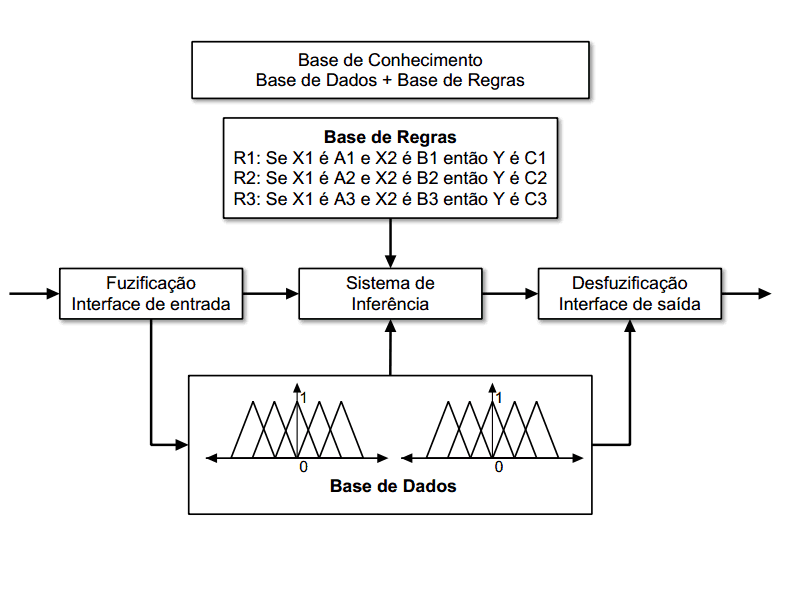
\includegraphics[width=0.9\textwidth]{sistema_nebuloso}
\end{figure}

Há duas formas básicas de se definir a base de regras de um SBRF: manual e automática. A definição manual depende inteiramente do conhecimento dos especialistas sobre o problema em questão, e por outro lado, na definição automática, são utilizados algoritmos para a construção das regras. Neste trabalho optamos por usar a forma automática, através do algoritmo proposto por \citeonline{wang1992generating}.

%A ideia central do método de Wang-Mendel é gerar regras fuzzy a partir de pares de dados numéricos, utilizando a modelagem das variáveis lingüísticas em conjuntos fuzzy, criando, assim, uma base comum de regras para o SBRF. Esse método é composto basicamente por 5 passos: 1) modelagem das variáveis linguísticas de entrada e de saída em conjuntos fuzzy e divisão dos dados em pares; 2) geração das regras a partir da modelagem do passo anterior; 3) Calculo de um grau para cada regra gerada; 4) remoção das regras conflitantes e 5) criação da base comum de regras fuzzy.

%A primeira etapa de modelagem das variáveis linguísticas é transforma-las em conjuntos fuzzy. Variáveis linguísticas podem ser "alto", "baixo", "medio", "neutro", "positivo", dentre outras. É nessa etapa que os projetistas do SBRF mapeiam essas variáveis em conjuntos fuzzy. Uma vez mapeadas as variáveis, os dados precisam ser divididos em pares, entrada e saída. Ao fim dessa etapa, têm-se um conjunto de dados numéricos, divididos em pares e mapeados para os conjuntos fuzzy. 

%A etapa seguinte, de geração de regras, é onde as primeiras regras são geradas. Cada par de dados origina uma regra fuzzy e essa regras são passadas para a próxima etapa. Na etapa 3 é onde se calcula os chamados graus de compatibilidade das regras. Nessa etapa, todas as regras geradas avaliam cada par de dados existentes, calculando o quanto compatível aquela regra é com o par de dados em questão. Após essa etapa, um valor numérico, chamado de grau de polaridade, é associado a cada regra avaliada  \cite{wang1992generating}.

%Uma vez geradas as regras e calculados os graus de compatibilidade, é preciso remover regras contraditórias e decidir entre regras iguais. É no quarto passo que é feita essa filtragem das regras. Na geração indiscriminada de regras, é comum surgirem regras que tenham antecedentes iguais e conseqüentes diferentes, como "Se a opinião é ALTA então ela é POSITIVA" e "Se a opinião é ALTA então ela é NEGATIVA". A decisão de qual regra utilizar é baseada no grau associado a cada regra. A que tiver o maior grau associado, é selecionada para a base final de regras. Além disso, regras repetidas (com antecedentes e conseqüentes idênticos) são também descartadas. Por fim, o último passo é a apresentação da base comum de regras geradas.

Existem vários modelos de sistemas fuzzy, sendo que a distinção entre eles se dá no consequente das regras. Entre os modelos mais conhecidos estão o Mamdani \cite{mamdani1975experiment}, que utiliza conjuntos fuzzy nos consequentes das regras, Takagi-Sugeno \cite{takagi1985fuzzy}, no qual o consequente é representado por uma função das variáveis de entrada, e o Tsukamot \cite{tsukamoto1979approach}, que utiliza funções de pertinência monotônicas no consequente. Dentre os poucos trabalhos encontrados que aplicam conceitos fuzzy em mineração de opinião, todos seguiram o modelo de Mamdani.

Para se determinar a saída de um SBRF é necessário definir um mecanismo de inferência fuzzy, que também é conhecido por Método de Raciocínio Fuzzy. Há dois métodos muito utilizados em sistemas de classificação fuzzy \cite{cintra2012genetic}, propostos por \citeonline{cordon1999proposal}, o Método de Raciocínio Fuzzy Geral (MRFG) e o Método de Raciocínio Fuzzy Clássico (MRFC).

O MRFC classifica um exemplo usando a regra que tem o maior grau de compatibilidade com o exemplo. Seja $e_p = (a_{p1}, a_{p2}, \cdots, a_{pm})$ um exemplo para ser classificado, e {$R_1,R_2, \cdots, R_s$} o conjunto de regras do sistema de classificação, cada uma com $m$ antecedentes e $A_{il_i}(a_{p_i}), i = 1, \cdots, m$, ser o grau de pertinência de uma característica $a_{p_i}$ para o conjunto fuzzy $i$ da regra $R_k$, o MRFC aplica os seguintes passos para classificar o exemplo $e_p$ \cite{cintra2012genetic}:

\begin{enumerate}
\item Calcula o grau de compatibilidade entre o exemplo $e_p$ e cada regra $R_k$, para $k = 1, \cdots, s$ e a norma \textbf{t}, através da equação \ref{eq:compat}:
\begin{equation}
Compat(R_k, e_p) = \textbf{t}(A_{1l_1}(a_{p_1}), A_{2l_2}(a_{p_2}), \cdots, A_{ml_m}(a_{p_m}))
\label{eq:compat}
\end{equation}
\item Encontra a regra $R_{kmax}$ que tem o maior grau de compatibilidade com o exemplo:
\begin{equation}
Compat(R_{kmax}, e_p) = max{Compat(R_k, e_p)}, k = 1,2, \cdots, s
\end{equation}
\item Associa a classe $c_j$ ao exemplo $e_p$, onde $c_j$ é a classe definida pela regra máxima $R_{kmax}$
\end{enumerate}

A figura \ref{fig:mrfc} ilustra esse processo.

\begin{figure}[H]  
  \caption{Método de Raciocínio Fuzzy Clássico (MRFC)}
  \label{fig:mrfc}
  \centering
    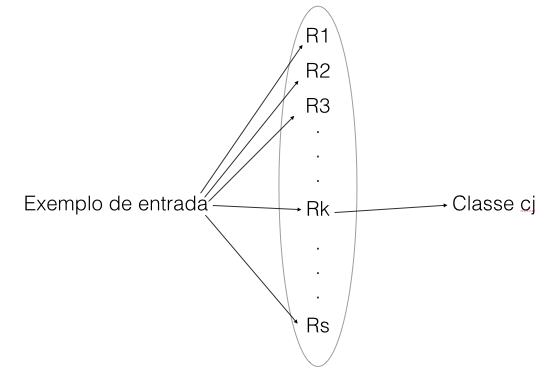
\includegraphics[width=0.7\textwidth]{mrfc}
\end{figure}

O MRFG, por outro lado, classifica um exemplo considerando todos os demais exemplos em relação as classes finais. Os seguintes passos mostram como MRFG funciona \cite{cintra2012genetic}:

\begin{enumerate}
\item De maneira similar ao MRFC, o MRFG calcula os graus de compatibilidade entre o exemplo $e_p$ e cada regra $R_k$, para $k = 1, \cdots, s$.
\item Calcula o valor de classificação $Class_c$, para cada classe. $Class_c$ é definida como a agregação dos graus de compatibilidade de todas as regras da classe $c_i$, e representa a compatibilidade do exemplo com todas as regras da classe $c_i$. Ele pode ser definido como:
\begin{equation}
Class_c = f{Compat(R_k, e_p)|c_i \, \acute{e}\, a\, classe\, da\, regra\, R_k}
\end{equation}
onde $f$ é o operador de agregação.
\item A classe com o maior grau é assinalada para o exemplo $e_p$.
\end{enumerate}

A figura \ref{fig:mrfg} ilustra esse processo.

\begin{figure}[H]  
  \caption{Método de Raciocínio Fuzzy Geral (MRFG)}
  \label{fig:mrfg}
  \centering
    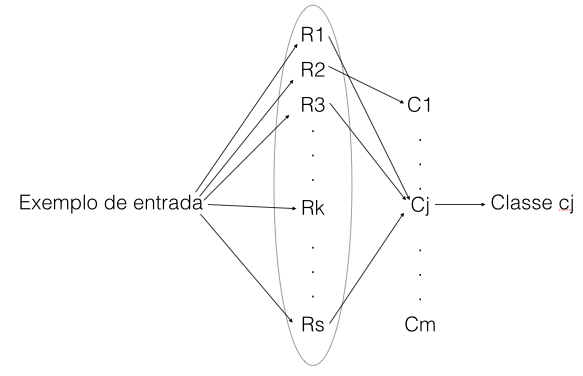
\includegraphics[width=0.7\textwidth]{mrfg}
\end{figure}

\section{Trabalhos relacionados}

Nesta seção serão discutidos trabalhos representativos e relacionados sobre mineração de opinião. É importante ressaltar novamente que poucos trabalhos foram encontrados na literatura sobre a aplicação de Lógica Fuzzy e extração de características de documentos para classificação de opinião. 

Um dos primeiros trabalhos a se destacar na área de mineração de opinião foi o de \citeonline{turney2002thumbs}, apresentando uma abordagem de classificação não supervisionada. Similar à tarefa de classificar documentos como positivos ou negativos, \citeonline{turney2002thumbs} propôs classificar opiniões como "recomendadas" (\textit{thumbs up} ou "não recomendadas" (\textit{thumbs down}). A classificação de um documento contendo as opiniões é feita através da média da polaridade do sentimento geral das opiniões das palavras num documento que continha adjetivos e advérbios. \citeonline{turney2002thumbs} conseguiu resultados de até 74\% em média entre os domínios que utilizou em sua pesquisa.

Paralelamente, \citeonline{pang2002thumbs} foi um dos primeiros a apresentar uma abordagem que utiliza técnicas clássicas de aprendizado de máquina para mineração de opinião. Eles compararam o desempenho entre os métodos \textit{Naive Bayes}, \textit{Maximum Entropy} e \textit{Support Vector Machine} (SVM). Esse trabalho mostrou que tais métodos produzem altas taxas de acurácia, alcançando 82,9\% de acurácia usando palavras isoladas (unigrams) com o SVM. Ainda mostraram que técnicas de aprendizado supervisionado produzem resultados melhores que técnicas de aprendizado não supervisionado. Contudo, a proposta apresentada por \citeonline{pang2002thumbs} é dependente do domínio utilizado, produzindo resultados muito ruins em outros tipos de dados, demandando outras rodadas de treinamento do classificador, aumentando custo e tempo para classificar os documentos.

Um pouco mais relacionados a esta pesquisa, os trabalhos de \citeonline{wilson2005recognizing}, \citeonline{taboada2008extracting}, e \citeonline{ohana2009sentiment} usaram um grande número de características dos documentos. Essas características envolveram desde a contagem de adjetivos e advérbios em frases e no documento inteiro, tuplas de palavras (bigrams e trigrams), como advérbios e adjetivos combinados, até a soma das polaridades dos n-grams, dentre outros. \citeonline{taboada2008extracting} e \citeonline{ohana2009sentiment} foram um dos poucos a apresentar o uso de dicionários de opiniões, nesse caso, o Sentiwordnet \cite{esuli2006sentiwordnet} que associa às palavras valores numéricos referentes as polaridades opiniativas. Na classificação de documentos como positivos ou negativos, estes trabalhos apresentaram 65,7\% de acurácia em \citeonline{wilson2005recognizing}, 80,6\% em \citeonline{taboada2008extracting} e 69,35\% em \citeonline{ohana2009sentiment}.

Em relação a aplicação da lógica fuzzy, nós encontramos o trabalho de \citeonline{nadali2010sentiment}. Ele propõe um modelo de lógica fuzzy para executar classificação de opinião de clientes em cinco classes: muito fraca, fraca, moderada, muito forte e forte. Além disso, ele apresentou uma metodologia que indica o uso de sistemas de inferência, conjuntos fuzzy que modelam as cinco classes mencionadas e a criação manual de regras fuzzy. Contudo, o artigo de \citeonline{nadali2010sentiment} não apresentou resultados ou qualquer discussão a respeito.

Outro trabalho encontrado foi o de \citeonline{ballhysa2012fuzzy} que propõe uma abordagem fuzzy para descobrir opiniões em postagens de blogs, determinando a polaridade do sentimento geral da postagem. Os autores apresentam conceitos fuzzy, como conjuntos fuzzy, operações entre conjuntos fuzzy, propõem um conjunto de medidas fuzzy e uma agregação fuzzy dessas medidas, embora um sistema fuzzy de inferência não seja utilizado. Contudo, as medidas fuzzy propostas parecem corresponder a medidas não fuzzy (\textit{crip}), mostrando que há, de fato, aplicação própria da lógica fuzzy no trabalho. Além disso, existe uma superficial descrição dos resultados obtidos de um conjunto de dados criados por eles mesmos e sem comparação com nenhum outro.

\citeonline{bing:2012} foi um dos poucos a apresentar um proposta fuzzy com resultados claros. Ele utiliza a lógica fuzzy  juntamente com ontologias de domínio para minerar opiniões de avaliações de produtos. Este trabalho aborda o problema da sobrecarga de informações que a web possui e a impossibilidade de catalogar as informações manualmente. Frente a essa motivação, o trabalho de \citeonline{bing:2012} apresenta um nova proposta oriunda da junção de conjuntos fuzzy e ontologias de domínio que os autores chamam de árvore de sentimentos de ontologias de domínios fuzzy (tradução livre de \textit{fuzzy domain ontology sentiment tree} - FDOST). Essa proposta extrai atributos de produtos das opiniões, constrói uma arvore de relacionamentos entre eles e, utilizando conjuntos fuzzy, classifica e associa os sentimentos. Dois são os conjuntos fuzzy utilizados neste trabalho: um conjunto de palavras de sentimentos e outro de palavras especificas do domínio (neste caso, \textit{laptops}). Eles são utilizados para construir o modelo da ontologia do domínio que, por sua vez, será utilizado para construir as árvores de relacionamento entre os atributos dos produtos e os sentimentos associados. Os resultados obtidos mostram que a utilização dos conjuntos fuzzy teve melhor desempenho que a mesma proposta sem o uso deles. 

E em \citeonline{mouthami2013sentiment} um novo algoritmo, chamado de Classificação de Sentimentos Fuzzy (da tradução livre de \textit{Sentiment Fuzzy Classification}), é proposto para melhorar a precisão da classificação de sentimentos de opiniões, utilizando lógica fuzzy, POS-Tags (\textit{Part of Speech Tags}) e uma base de dados de filmes como base de avaliação. Além do uso de lógica fuzzy, este trabalho contribui em mapear as etapas básicas do processo de mineração de opiniões, baseando-se nas tarefas executadas nos trabalhos relacionados descritos na pequisa dos autores. Conjuntos fuzzy são utilizados na etapa de classificação, onde são definidos três deles: conjunto fuzzy positivo, negativo e neutro. O trabalho,contudo, não apresentou resultados. 

Foi recorrente encontrar artigos com propostas de conceitos fuzzy pra mineração de opinião que não apresentavam resultados os discutiam apropriadamente - em alguns casos a metodologia nem era bem definida. Essa pesquisa difere destes e de outros trabalhos relacionados por apresentar e aplicar apropriadamente conceitos e técnicas fuzzy em mineração de opinião. Nós modelamos as variáveis fuzzy e construímos um sistema de inferência fuzzy baseado em características dos documentos. Nós executamos ainda nossos testes em conjuntos de dados já utilizados nos trabalhos relacionados, permitindo comparações diretas. Além disso, nós propomos uma fase de extração e seleção de características pouco encontradas em outros trabalhos, onde definimos, extraímos e selecionamos um grande número de características dos documentos, baseando-se nos poucos trabalhos que já fizeram esse tipo de extração.

O próximo capítulo apresenta a metodologia utilizada nessa pesquisa, descrevendo cada etapa realizada e as técnicas relevantes usadas nessas etapas.

\ifcsdef{mainfile}{}{\bibliography{pesquisa}}

\end{document}